% =============================================================================
%  Training neural networks with evolutionary algorithms
%  Report skeleton (pre Phase 6). All numbers are taken from docs/PROJECT_PLAN.md
%  (sections 4.1-4.4) and results/processed/; figures from ../figures/.
%  Text in \todo{...} still has to be written or checked. Compile: latexmk -pdf main.tex
% =============================================================================
\documentclass[11pt,a4paper]{article}

% ---------------------------------------------------------------- packages
\usepackage[T1]{fontenc}
\usepackage[utf8]{inputenc}
\usepackage{lmodern}
\usepackage{microtype}
\usepackage[margin=2.5cm]{geometry}
\usepackage{amsmath,amssymb,bm}
\usepackage{booktabs,multirow,tabularx,array}
\usepackage{graphicx}
\usepackage{subcaption}
\usepackage{xcolor}
\usepackage{enumitem}
\usepackage{algorithm}
\usepackage{algpseudocode}
\usepackage[numbers,sort&compress]{natbib}
\usepackage[colorlinks=true,linkcolor=blue!50!black,citecolor=green!40!black,urlcolor=blue!50!black]{hyperref}
\usepackage[nameinlink,capitalise]{cleveref}

\graphicspath{{../figures/}{figures/}}   % repo layout, or Overleaf with a figures/ folder
\setlist{itemsep=2pt,topsep=4pt}

% ---------------------------------------------------------------- macros
\newcommand{\todo}[1]{\par\noindent\fcolorbox{orange!80!black}{orange!10}{\parbox{\dimexpr\linewidth-2\fboxsep-2\fboxrule}{\small\textbf{TODO:} #1}}}
\newcommand{\todoinline}[1]{\textcolor{orange!80!black}{[\textbf{TODO:} #1]}}
\newcommand{\R}{\mathbb{R}}
\newcommand{\E}{\mathbb{E}}
\newcommand{\Ltr}{L_{\mathrm{train}}}
\newcommand{\clean}{\mathrm{MSE}_{\mathrm{clean}}}
\newcommand{\cmaes}{CMA-ES}
\newcommand{\lbfgs}{L-BFGS-B}
\newcommand{\nfloor}{\sigma^2}
\newcommand{\B}{B}

% =============================================================================
\title{Do Evolutionary Algorithms Train Neural Networks That Generalise Better?\\[4pt]
\large An equal-budget comparison with derivative-based methods across training-set sizes}
\author{Marta Mateu L\'opez \and Aram Abrahamyan\\[4pt]
\small Computational Intelligence (CI-MAI), Universitat Polit\`ecnica de Catalunya}
\date{November 2026}

\begin{document}
\maketitle

% =============================================================================
\begin{abstract}
Evolutionary algorithms (EAs) can train the weights of a neural network without gradients, and it is
often suggested that, by not following the gradient into the nearest sharp minimum, they find networks
that generalise better. We test this claim in a controlled setting: a one-hidden-layer perceptron
(41 weights) on a synthetic regression problem with a known noise-free target and noise floor
$\nfloor=0.09$, trained by two EAs (\cmaes{} and a real-coded genetic algorithm) and two
derivative-based methods (\lbfgs{} and mini-batch Adam) under the same budget of $10^5$
error-function evaluations, for training-set sizes $n\in\{25,100,400,1600\}$ and 30 paired seeds.
With the network of lowest training error, the GA has by far the lowest test error at $n\le 100$
(clean test MSE $0.030$ vs.\ $0.067$--$0.092$ at $n=100$) and the highest at $n=1600$, while \cmaes{}
behaves like the gradient methods. The GA, however, has the highest training error at every $n$:
its advantage is implicit early stopping, not a better optimum. When every method receives the same
realistic validation data (a selection set of $n$ points) to choose its early-stopping point and its
hidden-layer size, the advantage disappears: the GA is on par only at $n=25$ and worse from $n=100$ on,
\cmaes{} is on par with the gradient methods, and the gradient methods reach their best networks with
5--1000$\times$ fewer evaluations. GA solutions are flatter than \lbfgs{} solutions at equal training
error, but flatness does not predict test error except at $n=25$. The results are robust to the cost
assigned to a gradient, to a wall-clock budget and to a ten-fold larger GA budget.
\todoinline{final pass once the text is written; max.\ $\sim$200 words}
\end{abstract}

\tableofcontents
\clearpage

% =============================================================================
\section{Introduction}
\label{sec:intro}

\paragraph{Context.}
The application of evolutionary search to artificial neural networks is a long-standing research topic
\citep{yao1999evolving}. Evolution can act on the connection weights, the architecture (layers, units,
connectivity), the hyper-parameters, the activation functions and the learning rules. For weight
training, EAs have clear advantages over derivative-based methods: the error function does not need to be
continuous or differentiable, it may include discrete information (such as the number of units) and it
may be noisy. On the other hand, the error landscape is deceptive (similar networks can perform very
differently) and multimodal (permuting hidden units with their weights leaves the network unchanged), and
the computational cost is high \citep{yao1999evolving}.
\todo{1--2 sentences on the renewed interest (large-scale ES/GA for deep RL,
\citep{salimans2017evolution,such2017deep}) and why a small, controlled study is still informative.}

\paragraph{Research question.}
\begin{description}
  \item[RQ1] With the same computational budget, does an EA find networks that \emph{generalise} better than
  a derivative-based method, or only networks that \emph{fit} the training data as well?
  \item[RQ2] Does the answer depend on the size of the training sample?
\end{description}

\paragraph{Hypothesis.}
\textbf{H1}: since the EA does not follow the gradient into the nearest sharp minimum, its advantage (if
any) appears with small or noisy training samples and disappears with large ones.
H1 is \emph{falsified} if the EA's test error is never lower than the baseline's, if its advantage grows
with $n$, or if a lower test error comes purely from a higher training error (under-fitting rather than a
better minimum). To separate these cases we always report training and test error side by side.

\paragraph{Approach and contributions.}
\begin{itemize}
  \item A controlled comparison of two EAs (\cmaes, GA) and two derivative-based methods (\lbfgs, Adam) that
  share one network implementation, one weight box $[-5,5]^{41}$, one initialisation and one budget unit,
  with the training-set size as the single factor (\cref{sec:methods,sec:setup}).
  \item An evaluation-counting protocol that charges gradients, mini-batches and populations consistently,
  with sensitivity checks on the cost of a gradient and a wall-clock budget (\cref{sec:budget}).
  \item Equal-effort hyper-parameter tuning on training error, which avoids rewarding settings that win by
  under-fitting (\cref{sec:tuning}).
  \item Evidence that the EAs' apparent generalisation advantage is implicit early stopping: it vanishes once
  all methods get the same validation-based early stopping and capacity selection
  (\cref{sec:res-selection,sec:res-arch}), and flatness of the solutions does not explain test error
  (\cref{sec:res-sharpness}).
\end{itemize}

\paragraph{Outline.}
\Cref{sec:background} reviews related work, \cref{sec:methods} describes the problem, model and optimisers,
\cref{sec:setup} the experimental protocol, \cref{sec:results} the results, \cref{sec:discussion} discusses
them against RQ1, RQ2 and H1, and \cref{sec:limitations,sec:conclusion} give limitations and conclusions.
All decisions are listed with their justification in \cref{app:decisions}.

% =============================================================================
\section{Background and related work}
\label{sec:background}

\subsection{Evolving neural network weights}
\todo{Weight evolution: early GA work \citep{montana1989training}; the review of \citet{yao1999evolving}
(weights, architectures, learning rules; permutation problem; cost); topology and weight evolution (NEAT,
\citep{stanley2002neat}); large-scale ES and GA for deep networks
\citep{salimans2017evolution,such2017deep}. Point out that most comparisons do not equalise the budget or
control the training-set size.}

\subsection{Evolution strategies and genetic algorithms}
\todo{CMA-ES \citep{hansen2001completely,hansen2016tutorial}: sampling from $\mathcal{N}(\bm m,\sigma^2\bm C)$,
covariance and step-size adaptation, default population $\lambda = 4+\lfloor 3\ln p\rfloor$, invariance
properties; why it suits $p\approx 40$ (full covariance is cheap). Real-coded GA: tournament selection,
blend crossover BLX-$\alpha$ \citep{eshelman1993real}, Gaussian mutation, elitism; implementation in DEAP
\citep{fortin2012deap}.}

\subsection{Derivative-based training}
\todo{L-BFGS-B: quasi-Newton with limited memory and box constraints \citep{byrd1995limited,zhu1997algorithm};
full-batch, deterministic, very evaluation-efficient on small smooth problems. Mini-batch SGD and Adam
\citep{kingma2015adam}: the standard deep-learning optimiser; gradient noise as an implicit regulariser.}

\subsection{Generalisation, flat minima and early stopping}
\todo{Flat-minima argument \citep{hochreiter1997flat}; sharp minima and the large-batch generalisation gap
\citep{keskar2017large}; sharpness is not invariant to reparametrisation \citep{dinh2017sharp} (motivates our
scale-aware measure and matched comparison, D11); interpolation of noisy labels by over-parameterised
networks \citep{zhang2017understanding}; early stopping as regularisation
\citep{morgan1990generalization,prechelt1998early}. This frames the two competing explanations we test:
flatter minima vs.\ implicit early stopping.}

% =============================================================================
\section{Problem, model and methods}
\label{sec:methods}

\subsection{Synthetic regression problem}
\label{sec:data}
Inputs $\bm x=(x_1,x_2)$ are drawn uniformly from $[-1,1]^2$ and targets are
\begin{equation}
  y = f(\bm x) + \varepsilon,\qquad f(\bm x)=\sin(\pi x_1)+\sin(\pi x_2),\qquad
  \varepsilon\sim\mathcal{N}(0,\sigma^2),\ \sigma=0.3 .
  \label{eq:generator}
\end{equation}
Because the noise is independent of $\bm x$, the lowest achievable test MSE is the noise floor
$\nfloor=0.09$, and for any network $\hat f$,
\begin{equation}
  \E\big[(\hat f(\bm x)-y)^2\big] = \nfloor + \underbrace{\E\big[(\hat f(\bm x)-f(\bm x))^2\big]}_{\clean}.
  \label{eq:decomposition}
\end{equation}
We report the \emph{clean} test MSE (error against the noise-free $f$ on the test inputs, floor $0$) as the
main generalisation measure; it equals the excess test MSE in expectation and is less noisy.
Regression was chosen over classification because it gives an exact noise floor and a smooth error
measure, and because all methods can minimise the same loss (D1). $\sigma=0.3$ makes the problem
noisy enough for over-fitting to matter (D2).

\paragraph{Data sets.}
\begin{itemize}
  \item \textbf{Training sets.} For every run seed $s\in\{0,\dots,29\}$, one pool of 1600 points is drawn;
  the training set of size $n$ is its first $n$ points, so the sets are \emph{nested} and every method
  sees the same data for a given $(s,n)$. $n\in\{25,100,400,1600\}$ (factor 4) is the single
  experimental factor.
  \item \textbf{Validation and test sets.} 5000 points each, drawn once with a fixed data seed (10000) and
  identical for all runs. In the core experiment they are only measured, never used for training or
  selection.
  \item \textbf{Selection set (Phase 5, D10).} For model selection we add, per run, $n$ further points from
  an independent random stream, nested like the training sets: a realistic validation set as a user would
  have it (the 5000-point set is far larger than any training set).
\end{itemize}
\todo{Figure (optional): $f$ on $[-1,1]^2$ with one training set of each size overlaid.}

\subsection{Model}
\label{sec:model}
A multilayer perceptron with one hidden layer of $H=10$ $\tanh$ units and a linear output,
\begin{equation}
  \hat f(\bm x;\bm\theta) = \bm w_2^\top \tanh(\bm W_1^\top \bm x+\bm b_1)+b_2,
  \qquad \bm\theta=(\bm W_1,\bm b_1,\bm w_2,b_2)\in[-5,5]^{p},\quad p=H(d+2)+1=41 .
  \label{eq:mlp}
\end{equation}
The training loss is $\Ltr(\bm\theta)=\frac1n\sum_{i=1}^n(\hat f(\bm x_i;\bm\theta)-y_i)^2$.
All methods use \emph{one} numpy implementation (forward pass, loss, analytic gradient by manual
back-propagation, and a vectorised loss for a whole population), so they optimise exactly the same function
and evaluations are counted identically. The parameter-to-data ratio $p/n$ ranges from $1.64$ ($n=25$,
over-parameterised) to $0.026$ ($n=1600$). $H=10$ is within the suggested 5--20 and can represent $f$:
at $n=1600$ all methods but the GA reach a clean test MSE of about $0.002$ (D5). All methods start from
the same initial weights $\bm\theta_0\sim U(-0.5,0.5)^{p}$ per seed and are confined to the same box
$[-5,5]^p$ (the suggested default).

\subsection{Optimisers}
\label{sec:optimisers}
All four methods share one interface: they receive the counted objective (\cref{sec:budget}), the initial
weights and a seed, and run until the budget is exhausted. The returned network is the one with the lowest
training loss seen (D6). \Cref{tab:optimisers} summarises the tuned settings (\cref{sec:tuning}).

\begin{description}
  \item[\cmaes] (\texttt{cma} library) with box constraints, initial step size $\sigma_0$ and the default
  population $\lambda=15$. When a run stops (convergence criteria of \texttt{cma}), it restarts from new
  random weights until the budget is used. Each candidate costs one loss evaluation.
  \item[Genetic algorithm] (DEAP) on real vectors: population 100, one elite, tournament selection (size 3),
  blend crossover BLX-$\alpha$ ($p_c=0.7$, $\alpha=0.5$), Gaussian mutation ($p_m=0.2$ per child, per-gene
  probability $0.1$, $\sigma_{\mathrm{mut}}=0.03$), clipping to $[-5,5]$; only changed children are
  re-evaluated.
  \item[\lbfgs] (SciPy) full-batch with analytic gradients, memory $m=50$, $\texttt{ftol}=10^{-12}$; when
  it converges, it restarts from new random weights until the budget is used (otherwise the baseline
  would effectively get a smaller budget).
  \item[Adam] (own numpy implementation) with mini-batches of $b=\min(64,n)$, learning rate $0.01$,
  $\beta_1=0.9$, $\beta_2=0.999$, projection onto the box after every step; the full training loss is
  evaluated every 5 epochs (and charged) to select the returned network.
\end{description}

\begin{table}[t]
  \centering
  \caption{Optimiser settings used in all experiments (tuned in Phase 3, \cref{sec:tuning}); all methods
  use the same initial weights, the same box $[-5,5]^{41}$ and the same budget.}
  \label{tab:optimisers}
  \small
  \begin{tabularx}{\linewidth}{@{}l l X@{}}
    \toprule
    Method & Role & Settings (\textbf{bold} = tuned) \\
    \midrule
    \cmaes{} & EA & $\bm{\sigma_0=0.3}$, \textbf{population 15 (default)}, bounds handling of \texttt{cma}, restarts \\
    GA & EA & \textbf{pop.\ 100}, elitism 1, tournament 3, BLX-0.5 ($p_c=0.7$), Gaussian mutation
             $p_m=0.2$, \textbf{per-gene 0.1}, $\bm{\sigma_{\mathrm{mut}}=0.03}$, clipping \\
    \lbfgs{} & gradient & \textbf{memory 50}, $\bm{\texttt{ftol}=10^{-12}}$, random restarts \\
    Adam & gradient & $\bm{\eta=0.01}$, \textbf{batch 64} (capped at $n$), $\beta=(0.9,0.999)$, projection,
                      full loss every 5 epochs \\
    \bottomrule
  \end{tabularx}
\end{table}

\subsection{What is equalised: the budget}
\label{sec:budget}
The primary budget is the number of \emph{error-function evaluations}, $\B=10^5$, a unit that is
independent of hardware and implementation, reproducible, and natural for EAs (D3, D4). The cost model is:
\begin{itemize}
  \item one full training-loss evaluation costs 1; a population of $P$ candidates costs $P$;
  \item one loss-and-gradient call costs $g=2$: reverse-mode back-propagation costs 1.8--2.3 loss
  evaluations in our implementation (\cref{tab:gradcost}); $g=1$ and $g=3$ are tested (\cref{sec:res-robust});
  \item a mini-batch gradient on $b$ of the $n$ points costs $g\,b/n$, so one epoch costs one full gradient.
\end{itemize}
A counted-objective wrapper charges every call, refuses any call that would exceed $\B$, keeps the
best-so-far network and snapshots it at checkpoint evaluation counts (a 1-2-5 grid; 10 per decade in
Phase 5). A run cut at $B'<\B$ therefore returns exactly what a run with budget $B'$ would, which gives
convergence curves and results at smaller budgets for free. As a secondary budget we use \emph{wall-clock
time} with one limit per $n$ (\cref{sec:res-robust}).

\begin{algorithm}[t]
  \caption{Counted objective shared by all methods (sketch).}
  \label{alg:budget}
  \begin{algorithmic}[1]
    \Function{Charge}{$c$} \Comment{$c$ = cost of the requested call}
      \If{$\textit{used}+c>\B$} \textbf{raise} BudgetExhausted \EndIf
      \State $\textit{used}\gets\textit{used}+c$
    \EndFunction
    \Function{Loss}{$\bm\theta$}: \Call{Charge}{1}; $\ell\gets\Ltr(\bm\theta)$; \Call{Record}{$\bm\theta,\ell$}; \Return $\ell$ \EndFunction
    \Function{LossGrad}{$\bm\theta$}: \Call{Charge}{$g$}; \Return $(\Ltr,\nabla\Ltr)(\bm\theta)$ \EndFunction
    \Function{Record}{$\bm\theta,\ell$}
      \If{$\ell<\ell^\ast$} $(\ell^\ast,\bm\theta^\ast)\gets(\ell,\bm\theta)$ \EndIf
      \State snapshot $\bm\theta^\ast$ at every checkpoint passed by this call
    \EndFunction
  \end{algorithmic}
\end{algorithm}

\begin{table}[t]
  \centering
  \caption{Measured cost of one loss-and-gradient call relative to one loss call (41 weights, mean of 3000 calls).}
  \label{tab:gradcost}
  \begin{tabular}{@{}lcccc@{}}
    \toprule
    $n$ & 25 & 100 & 400 & 1600 \\
    \midrule
    ratio & 2.26 & 2.15 & 1.91 & 1.81 \\
    \bottomrule
  \end{tabular}
\end{table}

\subsection{Model selection inside a run}
\label{sec:selection}
\begin{itemize}
  \item \textbf{Core (Phase 4):} the returned network is the one with the lowest training loss within the
  budget, the same rule for every method (D6). No early stopping: this isolates the question of what kind of
  minimum each optimiser finds.
  \item \textbf{Fair early stopping (Phase 5.1):} among the checkpoints of a run, the one with the lowest
  MSE on the selection set (D10).
  \item \textbf{Capacity and early stopping (Phase 5.3):} one run per $H\in\{2,4,6,10,15,20\}$, each with the
  full budget; the (H, checkpoint) pair with the lowest selection MSE is returned. The selection set only
  chooses among networks whose weights were fitted on the training set.
\end{itemize}

% =============================================================================
\section{Experimental setup}
\label{sec:setup}

\subsection{Design}
\begin{table}[h]
  \centering
  \caption{Experiments. Seeds are paired across methods (same training set and initial weights).}
  \label{tab:design}
  \small
  \begin{tabularx}{\linewidth}{@{}l l X r@{}}
    \toprule
    Phase & Experiment (config) & Content & Runs \\
    \midrule
    3 & Tuning (\texttt{tuning.yaml}) & 9--15 settings per method, seeds 100--104, $n\in\{100,400\}$ & 420 \\
    3 & Checks (\texttt{core.yaml}) & tuned settings, seeds 100--104, all $n$ & 80 \\
    4 & Core sweep (\texttt{core.yaml}) & 4 methods $\times$ 4 $n$ $\times$ 30 seeds, $\B=10^5$ evaluations & 480 \\
    4 & Wall-clock (\texttt{core\_wallclock.yaml}) & same, time limit 4/4/7/12\,s per $n$, serial & 480 \\
    4 & GA long (\texttt{core\_ga\_long.yaml}) & GA only, $10^6$ evaluations, seeds 0--9 & 40 \\
    4 & Gradient cost (\texttt{core\_gradcost\{1,3\}.yaml}) & \lbfgs{} and Adam with $g=1$ and $g=3$ & 480 \\
    5.1/5.2 & Selection (\texttt{p5\_selection.yaml}) & core + selection set, dense checkpoints, saved weights & 480 \\
    5.3 & Capacity (\texttt{p5\_arch.yaml}) & $H\in\{2,4,6,15,20\}$ (+ $H=10$ from 5.1) & 2400 \\
    \bottomrule
  \end{tabularx}
\end{table}

\subsection{Random streams and seeds}
Run seeds $0$--$29$ (evaluation) and $100$--$104$ (tuning, never used for evaluation). The training data
use the run seed directly; initial weights, optimiser randomness and selection sets use independent
streams derived from (seed, stream), so the initial weights never reuse the random numbers that drew the
training points (D7, D8). Validation and test sets use a separate data seed.

\subsection{Hyper-parameter tuning}
\label{sec:tuning}
Every method gets the same tuning effort (D9): a grid of 8 settings (\cref{tab:grids}), run on the tuning
seeds at $n\in\{100,400\}$ with the full budget; the winner has the lowest mean rank of the final
\emph{training} MSE over the (seed, $n$) cells. Tuning on validation error would reward settings that win by
under-fitting (a hidden form of early stopping), so each method is instead made as good an
\emph{optimiser} as it can be. One pre-registered extension round was applied to every method: a winner at the
edge of an ordered parameter received one step past that edge, and winners were re-ranked over both rounds
(\cmaes{} 9, GA 15, \lbfgs{} 9, Adam 9 settings in total).

\begin{table}[t]
  \centering
  \caption{Tuning grids (round 1 $\times$ round 2 edge extension) and winners.}
  \label{tab:grids}
  \small
  \begin{tabularx}{\linewidth}{@{}l X X l@{}}
    \toprule
    Method & Round 1 grid & Edge extension & Winner \\
    \midrule
    \cmaes{} & $\sigma_0\in\{0.1,0.3,0.5,1\}\times\lambda\in\{15,50\}$ & $\lambda=8$ & $\sigma_0=0.3$, $\lambda=15$ \\
    GA & $\sigma_{\mathrm{mut}}\in\{0.1,0.3\}\times$ per-gene $\{0.1,0.3\}\times$ pop.\ $\{50,100\}$
       & $\sigma_{\mathrm{mut}}=0.03$, per-gene $0.03$, pop.\ 200 & $0.03$, $0.1$, 100 \\
    \lbfgs{} & $m\in\{5,10,20,50\}\times\texttt{ftol}\in\{\text{default},10^{-12}\}$ & $m=100$ & $m=50$, $10^{-12}$ \\
    Adam & $\eta\in\{0.001,0.003,0.01,0.03\}\times b\in\{16,64\}$ & $b=128$ & $\eta=0.01$, $b=64$ \\
    \bottomrule
  \end{tabularx}
\end{table}

\subsection{Measurements}
Each run stores its configuration, code version (git commit), budget used, wall time, the returned network
and its metrics (training, validation and test MSE, clean test MSE, generalisation gap, share of weights at
the bounds, weight norm), a convergence curve (all metrics of the best-so-far network at every checkpoint),
the best-validation checkpoint and per-restart results. Phase 5 additionally stores the selection-set MSE and
the weights at every checkpoint.

\subsection{Sharpness (Phase 5.2)}
\label{sec:sharpness-def}
Two measures of how sharp $\Ltr$ is around $\bm\theta$ (D11):
\begin{align}
  S_\rho(\bm\theta) &= \frac1K\sum_{k=1}^{K}\Ltr(\bm\theta+\bm\epsilon_k)-\Ltr(\bm\theta),
  \qquad \|\bm\epsilon_k\| = \rho\,\|\bm\theta\|,\ \rho=0.01,\ K=200, \label{eq:sharp}\\
  \lambda_{\max}(\bm\theta) &= \text{largest eigenvalue of the Hessian }\nabla^2\Ltr(\bm\theta)\in\R^{41\times41}, \nonumber
\end{align}
The Hessian is computed by central differences of the analytic gradient.
$S_\rho$ (primary) uses a perturbation radius relative to the weight norm, because $\lambda_{\max}$ grows
with the weight scale \citep{dinh2017sharp} and the methods reach very different weight norms. Sharpness
also depends on how far training has gone, so the methods are compared at \emph{matched training error}: for
each seed, the first checkpoint of \cmaes, \lbfgs{} and Adam whose training MSE is down to the GA's final
training MSE.

\subsection{Statistics}
For each $n$, methods are compared on the clean test MSE with the paired Wilcoxon signed-rank test
\citep{wilcoxon1945individual} over the 30 seeds, for all 6 method pairs at all 4 sizes (24 tests), with
Holm's correction over the 24 tests \citep{holm1979simple} and Cliff's $\delta$ as effect size
\citep{cliff1993dominance} (see also \citep{demsar2006statistical}). We report medians and inter-quartile
ranges; significance means $p_{\mathrm{Holm}}<0.05$. Secondary experiments are compared with the core sweep
seed by seed.

\subsection{Implementation and reproducibility}
Python 3.14, numpy \citep{harris2020array}, SciPy \citep{virtanen2020scipy}, \texttt{cma} 4.5.0, DEAP 1.4.4
\citep{fortin2012deap}; 169 unit tests (gradient check, budget accounting, determinism, statistics).
Every run is determined by (config, method, $n$, seed) and stores the git commit; raw results are one JSON
file per run, aggregated tables are versioned. \Cref{app:repro} lists the commands and commits.
\todoinline{hardware (Mac, 11 cores), total compute time; link to the repository}

% =============================================================================
\section{Results}
\label{sec:results}

\subsection{Budget, tuning and convergence checks}
\label{sec:res-checks}
\paragraph{Budget.} In a pilot (3 seeds) the training MSE of \cmaes{} changes by less than 1\% between $5\cdot10^4$
and $10^5$ evaluations for $n\ge100$, while at $2\cdot10^4$ it is still 4--8\% above its plateau; hence
$\B=10^5$. The pilot already showed the central effect: at $n=100$ the clean test MSE of \cmaes{}
\emph{rises} with the budget, from $0.039$ at $10^4$ to $0.072$ at $10^5$ evaluations, i.e.\ an under-converged
optimiser looks as if it generalised better.
\todo{Table with the pilot budget curve (PROJECT\_PLAN §4.1) or move it to the appendix.}

\paragraph{Convergence with the tuned settings.} \Cref{tab:checks}. \cmaes, \lbfgs{} and Adam have levelled off
by $10^5$ evaluations (the training MSE improves by $\le1.3\%$ over the second half of the budget for $n\ge400$),
and at $n=25$ all three interpolate the training data. The GA has \emph{not} levelled off: its training MSE
stays above the noise floor for $n\ge400$ and still falls by 7--9\% over the second half.
5--17\% of the weights of \cmaes, \lbfgs{} and Adam sit at the bounds $\pm5$, but almost none of the GA's.

\begin{table}[t]
  \centering
  \caption{Checks with the tuned settings (seeds 100--104, $10^5$ evaluations): median training MSE, its
  relative decrease over the second half of the budget (in brackets) and the share of weights at $\pm5$.}
  \label{tab:checks}
  \small
  \begin{tabular}{@{}r cccc c@{}}
    \toprule
    $n$ & \cmaes & GA & \lbfgs & Adam & at bounds (C/G/L/A) \\
    \midrule
    25   & 0.0000         & 0.053 (21\%)  & 0.0000         & 0.0000         & 10/2/5/7\,\% \\
    100  & 0.058 (7.2\%)  & 0.096 (9.0\%) & 0.051 (0.7\%)  & 0.058 (3.2\%)  & 12/0/17/10\,\% \\
    400  & 0.086 (1.3\%)  & 0.103 (7.6\%) & 0.083 (0.4\%)  & 0.085 (0.6\%)  & 7/0/10/10\,\% \\
    1600 & 0.087 (0.3\%)  & 0.101 (7.1\%) & 0.086 (0.2\%)  & 0.088 (0.0\%)  & 5/0/7/2\,\% \\
    \bottomrule
  \end{tabular}
\end{table}

\subsection{Core comparison at equal evaluations}
\label{sec:res-core}
\Cref{tab:core,fig:core} give training and clean test MSE of the returned networks (lowest training loss).

\begin{table}[t]
  \centering
  \caption{Core sweep ($10^5$ evaluations, 30 seeds): median training MSE / clean test MSE of the returned
  network. Bold: not significantly worse than the best method at that $n$ (Wilcoxon, Holm over 24 tests).
  Noise floor of the training MSE: $0.09$; floor of the clean test MSE: $0$.}
  \label{tab:core}
  \small
  \begin{tabular}{@{}r cccc@{}}
    \toprule
    $n$ & \cmaes & GA & \lbfgs & Adam \\
    \midrule
    25   & 0.000 / 1.85           & 0.036 / \textbf{0.149} & 0.000 / 2.26   & 0.000 / 1.69 \\
    100  & 0.054 / 0.067          & 0.082 / \textbf{0.030} & 0.045 / 0.092  & 0.052 / 0.070 \\
    400  & 0.079 / \textbf{0.011} & 0.095 / 0.014          & 0.078 / 0.014  & 0.080 / \textbf{0.011} \\
    1600 & 0.088 / \textbf{0.0023}& 0.101 / 0.012          & 0.088 / 0.0027 & 0.089 / \textbf{0.0024} \\
    \bottomrule
  \end{tabular}
\end{table}

\begin{figure}[t]
  \centering
  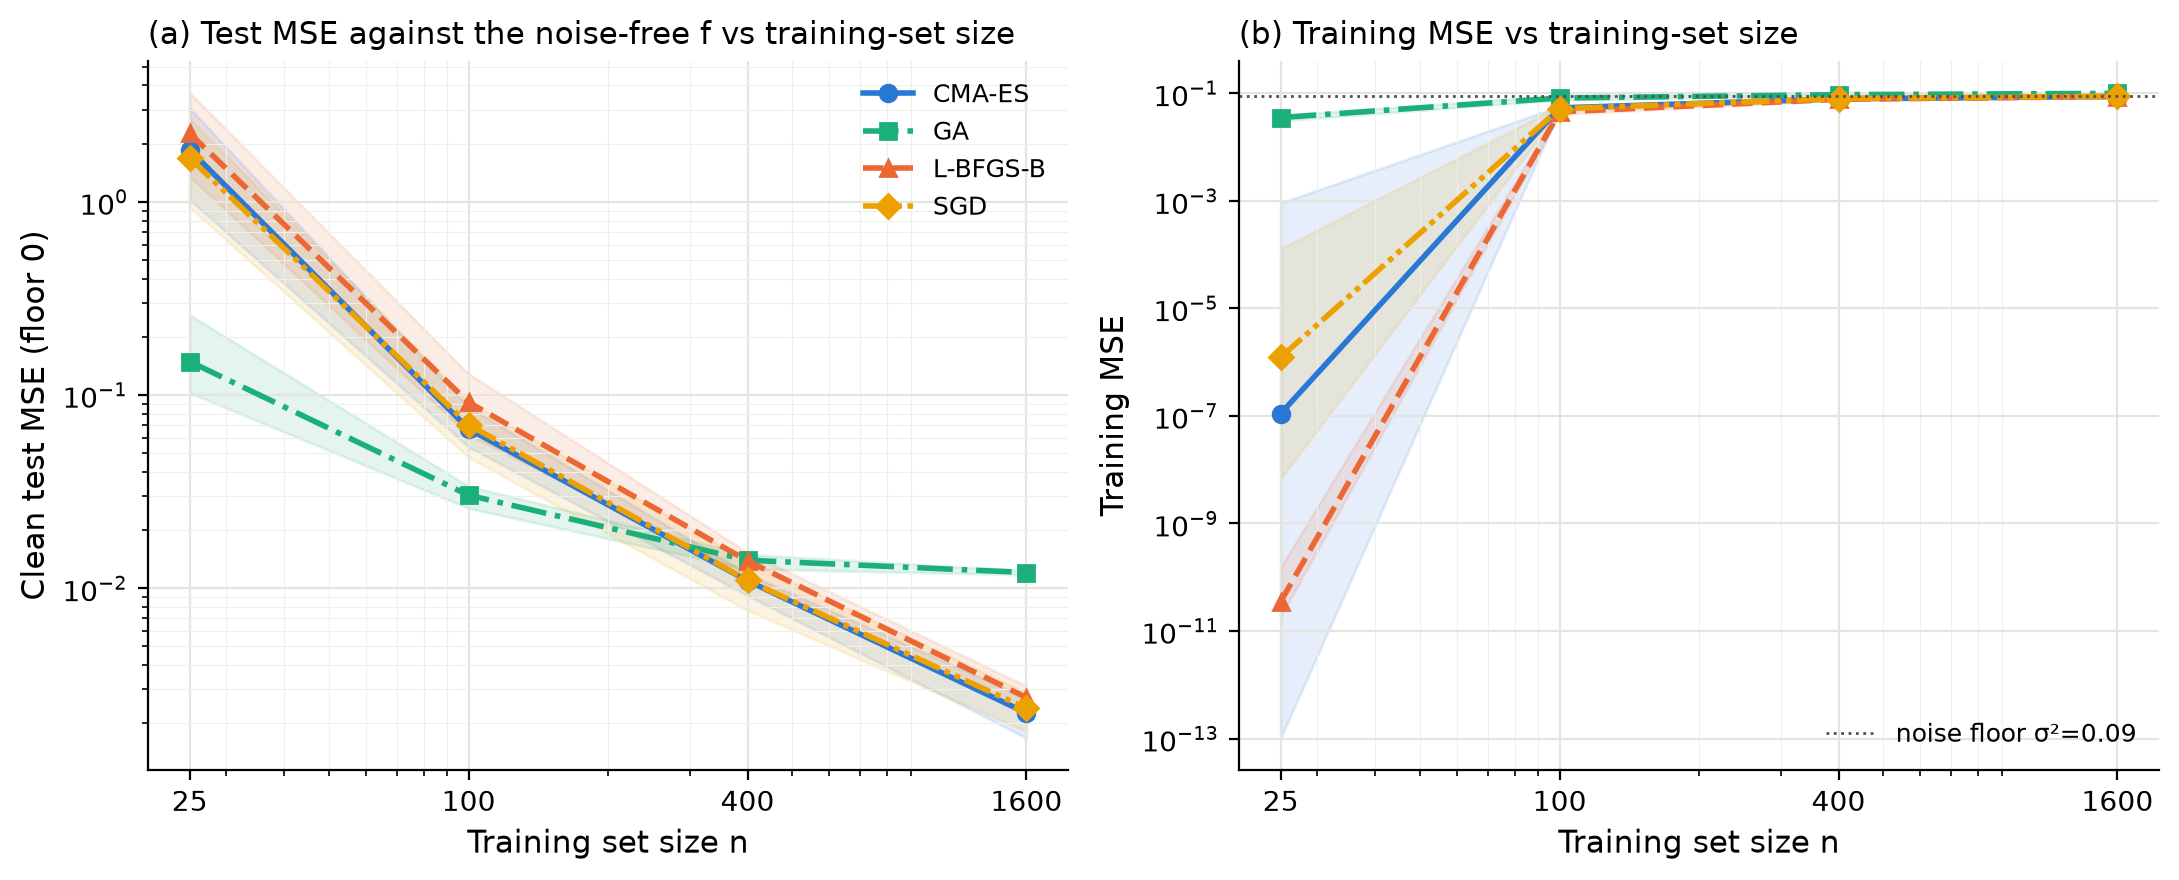
\includegraphics[width=\linewidth]{fig1_test_train_vs_n.png}
  \caption{Core sweep: (a) clean test MSE and (b) training MSE of the returned networks vs.\ training-set size
  (median and inter-quartile range over 30 seeds; log--log). \todoinline{panel (b): the log axis down to
  $10^{-13}$ (interpolation at $n=25$) hides the GA's higher training MSE at $n\ge100$; use a broken or linear axis}}
  \label{fig:core}
\end{figure}

\begin{itemize}
  \item $n\le100$: the GA beats every other method by a wide margin (Cliff's $\delta\approx0.95$--$0.98$,
  $p_{\mathrm{Holm}}<10^{-7}$). Among the other three only Adam vs.\ \lbfgs{} differ at $n=100$.
  \item $n=400$: \cmaes{} and Adam (equal) beat the GA and \lbfgs{} ($p_{\mathrm{Holm}}\le0.005$).
  \item $n=1600$: the GA is the worst method ($\delta=1$ against all), \cmaes{} beats \lbfgs.
  \item The GA has the highest training MSE at every $n$ (above the noise floor for $n\ge400$): its small-$n$
  advantage comes together with fitting less, and turns into a disadvantage once fitting more no longer
  over-fits. Among the other three the same pattern holds: \lbfgs{} fits hardest and generalises worst of them.
  \item At $n=25$, \cmaes, \lbfgs{} and Adam interpolate the noisy training data (training MSE $\approx0$)
  and their clean test MSE is $20\times$ the noise floor.
\end{itemize}

\begin{figure}[t]
  \centering
  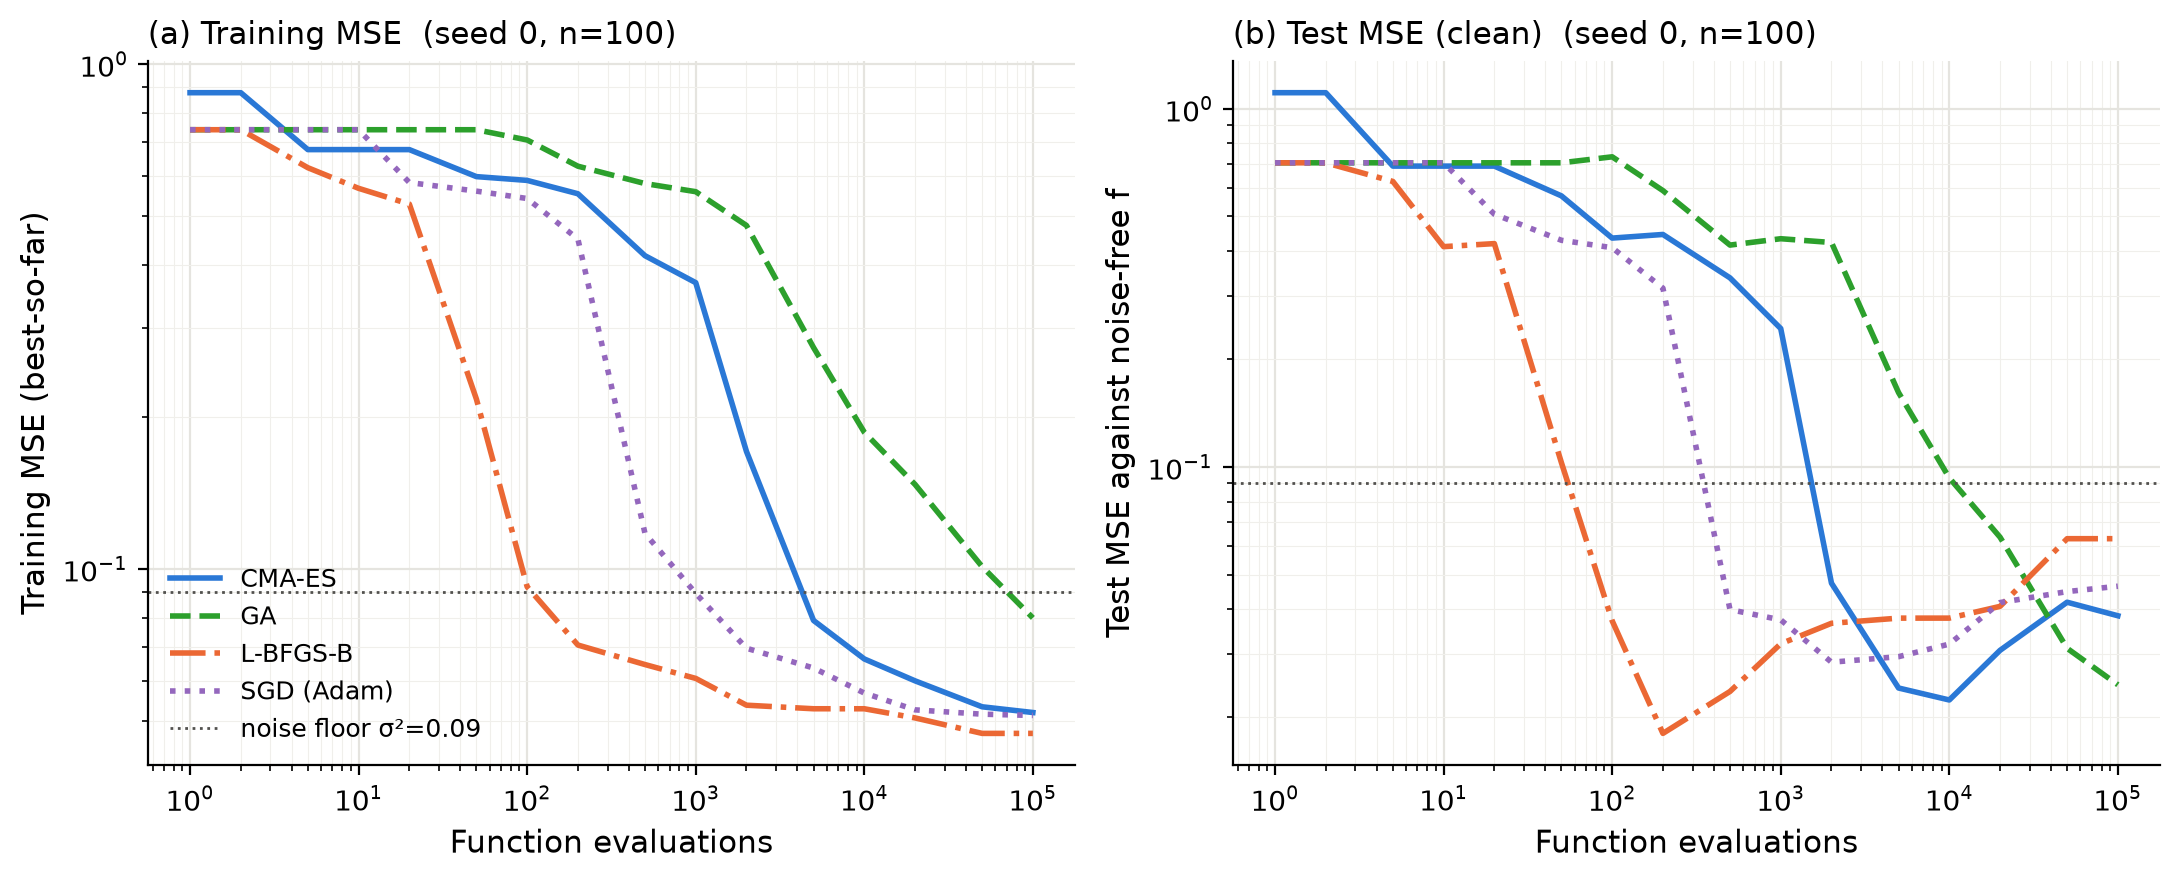
\includegraphics[width=\linewidth]{fig4_convergence_seed0_n100.png}
  \caption{Convergence of the best-so-far network (seed 0, $n=100$): (a) training MSE, (b) clean test MSE vs.\
  evaluations. \lbfgs{} reaches its lowest test error after about 200 evaluations and then over-fits;
  the GA is still improving on the training set at $10^5$.}
  \label{fig:convergence}
\end{figure}

\begin{figure}[t]
  \centering
  \begin{subfigure}{0.49\linewidth}
    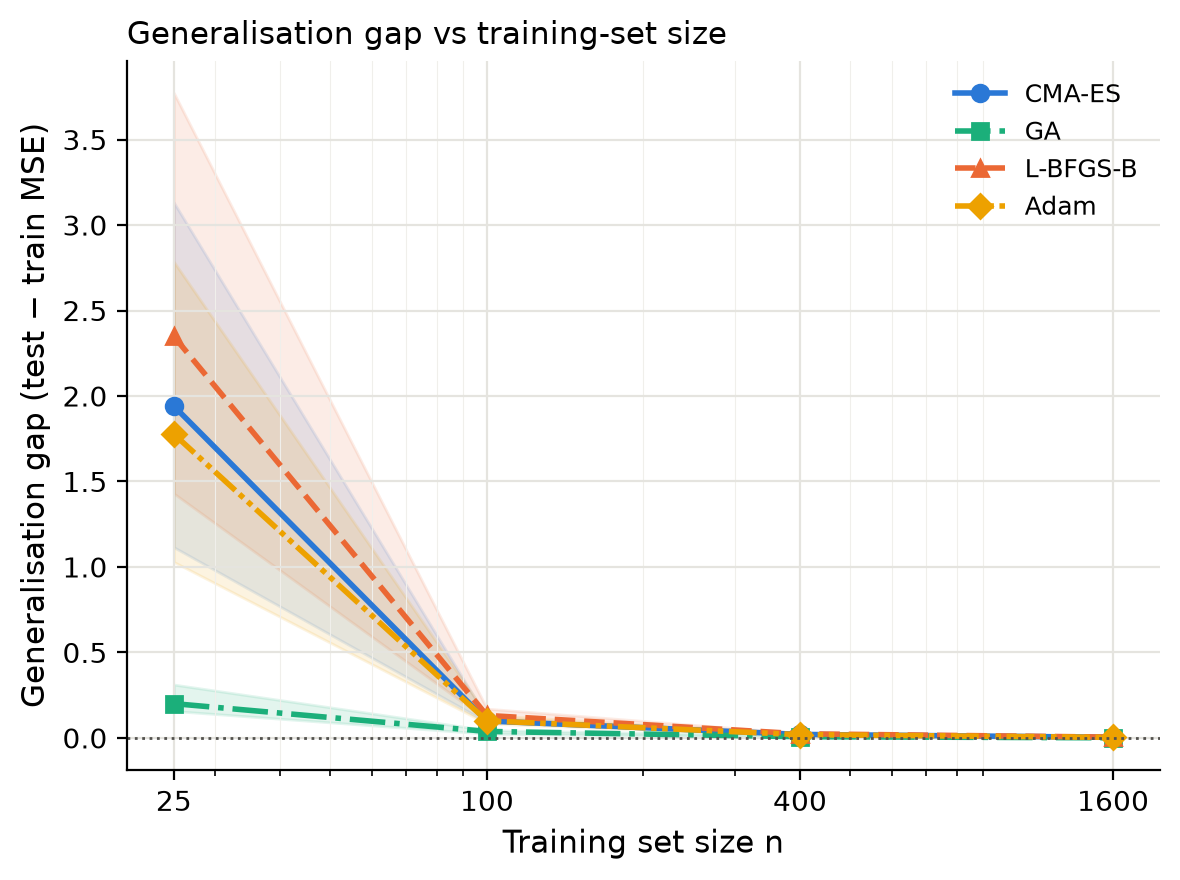
\includegraphics[width=\linewidth]{fig2_gap_vs_n.png}
    \caption{Generalisation gap (test $-$ train MSE).}
  \end{subfigure}\hfill
  \begin{subfigure}{0.49\linewidth}
    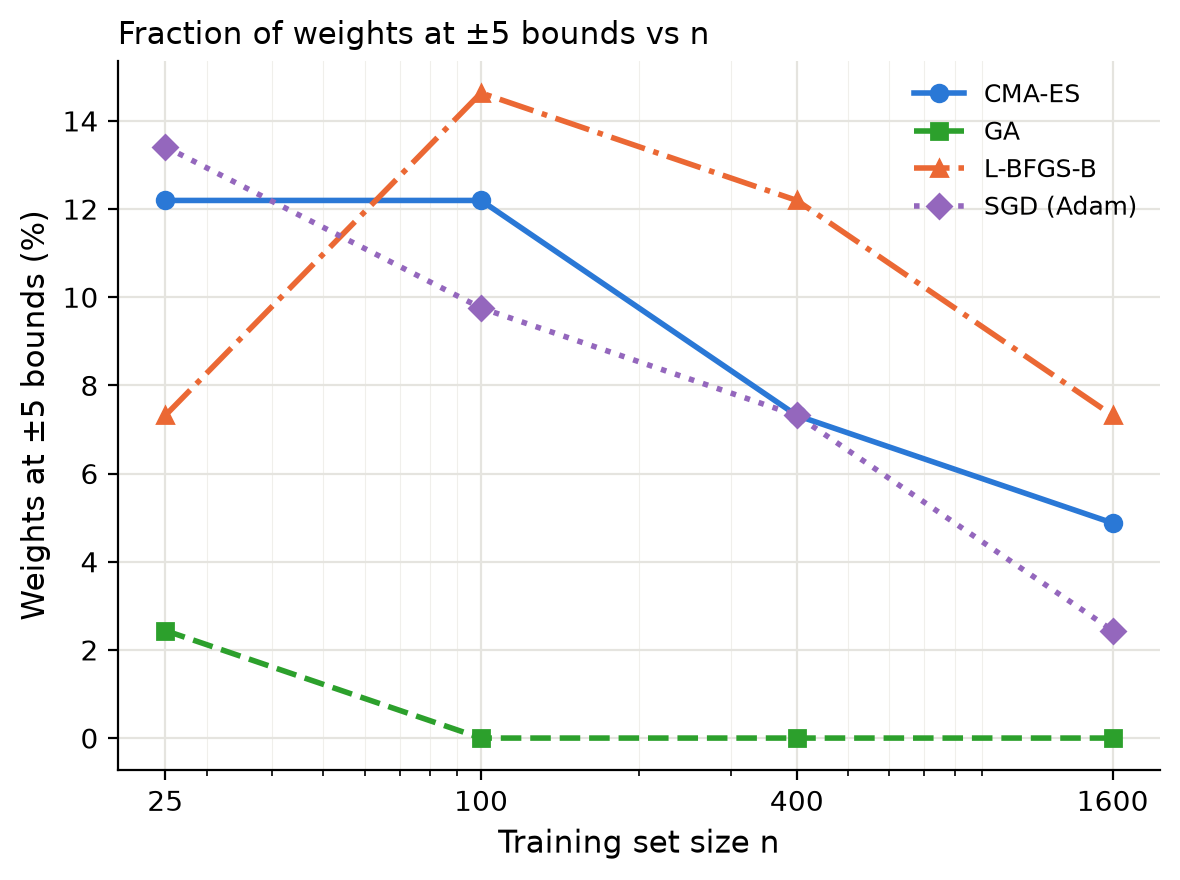
\includegraphics[width=\linewidth]{fig3_bounds_vs_n.png}
    \caption{Weights at the bounds $\pm5$.}
  \end{subfigure}
  \caption{Core sweep. \todoinline{(a): linear axis, $n=25$ flattens the rest; use log or symlog}}
  \label{fig:gap-bounds}
\end{figure}

\subsection{Robustness of the core result}
\label{sec:res-robust}

\paragraph{Ten-fold budget for the GA.} \Cref{tab:galong}. With $10^6$ evaluations (seeds 0--9) the GA fits
more, its large-$n$ disadvantage mostly disappears and at $n=25$ it starts to over-fit. It still fits less than
the other methods at every $n$ (training MSE $0.071$ vs.\ $0.043$--$0.052$ at $n=100$), i.e.\ it never reaches
the situation ``fits as well, generalises better''.

\begin{table}[t]
  \centering
  \caption{GA at $10^5$ vs.\ $10^6$ evaluations (seeds 0--9, paired) and Cliff's $\delta$ of the GA at $10^6$
  against the other methods at $10^5$ (clean test MSE; $\delta<0$: GA better; descriptive, 10 seeds).
  $^{*}$ change significant, $p_{\mathrm{Holm}}=0.008$ (paired Wilcoxon over 4 tests).}
  \label{tab:galong}
  \small
  \begin{tabular}{@{}r cc c@{}}
    \toprule
    $n$ & train MSE $10^5\to10^6$ & clean test MSE $10^5\to10^6$ & $\delta$ vs.\ \cmaes{} / \lbfgs{} / Adam \\
    \midrule
    25   & $0.037\to0.014$ & $0.138\to0.269^{*}$ (worse) & $-0.92$ / $-0.90$ / $-0.96$ \\
    100  & $0.087\to0.071$ & $0.029\to0.028$ (n.s.) & $-0.82$ / $-0.90$ / $-0.88$ \\
    400  & $0.098\to0.088$ & $0.015\to0.007^{*}$ (better) & $-0.70$ / $-0.92$ / $-0.62$ \\
    1600 & $0.099\to0.090$ & $0.012\to0.003^{*}$ (better) & $+0.62$ / $+0.26$ / $+0.50$ \\
    \bottomrule
  \end{tabular}
\end{table}

\paragraph{Cost of a gradient.} With $g=1$ or $g=3$ instead of $2$, \lbfgs{} and Adam change by at most a few
percent; no difference is significant except Adam at $n=100$ with $g=3$ (fewer steps, clean test MSE
$0.070\to0.065$, $p_{\mathrm{Holm}}=0.015$). The ranking is unchanged for $g=1$ and changes only by a
non-significant swap of \cmaes{} and Adam at $n=100$ for $g=3$; 23 of 24 pairwise verdicts are unchanged in
both cases. The choice $g=2$ does not drive the conclusions (D3).

\paragraph{Wall-clock budget.} With a time limit per $n$ (the median over methods of the serial time of a
$10^5$-evaluation run: 4, 4, 7, 12\,s) the GA, cheapest per evaluation, reaches $1.3$--$1.8\times$ more
evaluations (127k--180k), \cmaes{} and \lbfgs{} about the same, Adam 365k at $n=25$ but only 42k at $n=1600$
(many small steps). \cmaes, \lbfgs{} and Adam do not change significantly; the GA fits a bit more, so its test
MSE drops at $n\ge100$ (e.g.\ $0.014\to0.011$ at $n=400$) and rises at $n=25$. 19 of 24 verdicts are unchanged;
at $n=400$ the GA moves level with \cmaes{} and Adam. The same picture as with the longer GA budget.
\todo{Small table: evaluations reached per method and $n$ under the time limit.}

\subsection{Fair early stopping on a realistic validation set}
\label{sec:res-selection}
In the core sweep only the GA stops ``early'': it never reaches the over-fitting stage. Phase 5.1 gives every
method the same early stopping: the checkpoint with the lowest MSE on a selection set of $n$ points
(\cref{tab:es,fig:es}). Training is unchanged (the final networks are identical to the core sweep in all
480 runs).

\begin{table}[t]
  \centering
  \caption{Early stopping on the selection set (30 seeds): median clean test MSE of the selected checkpoint and
  median evaluations at that checkpoint. Bold: not significantly worse than the best method at that $n$.}
  \label{tab:es}
  \small
  \begin{tabular}{@{}r cccc@{}}
    \toprule
    $n$ & \cmaes & GA & \lbfgs & Adam \\
    \midrule
    25   & \textbf{0.129} (4.0k)  & \textbf{0.116} (20k)  & \textbf{0.117} (100) & \textbf{0.148} (1.4k) \\
    100  & \textbf{0.032} (10k)   & \textbf{0.031} (100k) & \textbf{0.024} (158) & \textbf{0.027} (3.2k) \\
    400  & \textbf{0.0052} (13k)  & 0.014 (100k)          & \textbf{0.0057} (251) & 0.0065 (4.0k) \\
    1600 & \textbf{0.0012} (20k)  & 0.012 (100k)          & \textbf{0.0013} (500) & 0.0018 (3.2k) \\
    \bottomrule
  \end{tabular}
\end{table}

\begin{figure}[t]
  \centering
  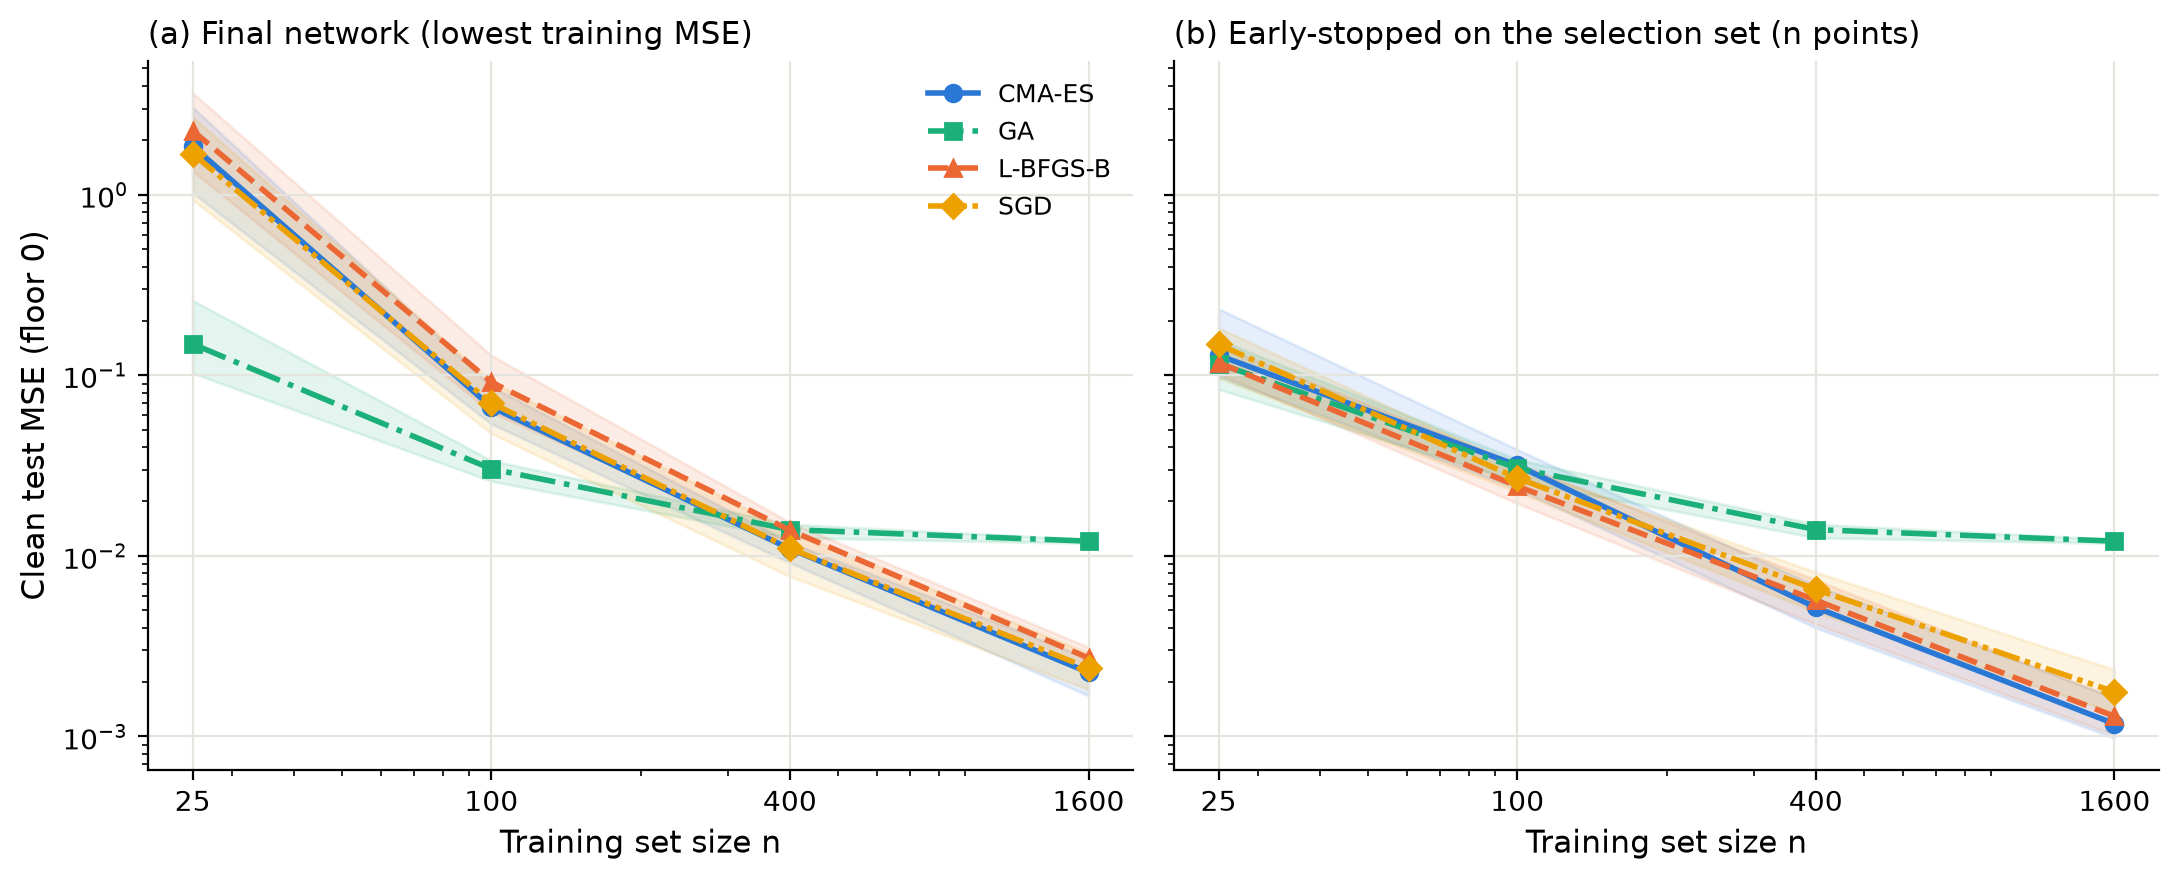
\includegraphics[width=\linewidth]{fig5_early_stopping_vs_n.png}
  \caption{Clean test MSE vs.\ $n$: (a) returned network (lowest training MSE), (b) early-stopped on the
  selection set of $n$ points.}
  \label{fig:es}
\end{figure}

\begin{itemize}
  \item The GA's small-$n$ advantage disappears: no significant difference at $n=25$; at $n=100$ no method
  differs from the best (\lbfgs), but Adam beats the GA ($p_{\mathrm{Holm}}=0.011$); at $n\ge400$ the GA is
  the worst ($\delta\ge0.95$).
  \item The gradient methods reach their best networks very early (\lbfgs{} after 100--500 evaluations, Adam
  1.4k--4k, \cmaes{} 4k--20k); the GA needs the whole budget for $n\ge100$.
\end{itemize}

\subsection{Sharpness of the solutions}
\label{sec:res-sharpness}
\Cref{fig:sharp} compares the methods at the GA's training MSE (\cref{sec:sharpness-def}).
\begin{itemize}
  \item Perturbation sharpness ($\times10^{-3}$): \lbfgs{} 4.2--5.5, \cmaes{} 2.6--3.1, GA 1.9--2.4, Adam
  2.0--2.3. The GA is flatter than \lbfgs{} at every $n$ ($p_{\mathrm{Holm}}\le4\cdot10^{-5}$) and than \cmaes{}
  at $n=100$ and $1600$; GA and Adam are about equal.
  \item Flatness does not predict generalisation: at $n\ge100$ the sharpest method (\lbfgs) has the lowest test
  MSE of the matched networks (e.g.\ $0.010$ vs.\ GA $0.014$ at $n=400$). Only at $n=25$ do the flatter networks
  (GA, Adam) also generalise better (GA $0.149$ vs.\ \lbfgs{} $0.237$).
  \item The returned networks differ far more (perturbation sharpness GA $0.002$ vs.\ $0.005$--$0.044$; weight
  norm 7--9 vs.\ 13--20), but this reflects training progress: the other methods keep fitting the noise.
\end{itemize}

\begin{figure}[t]
  \centering
  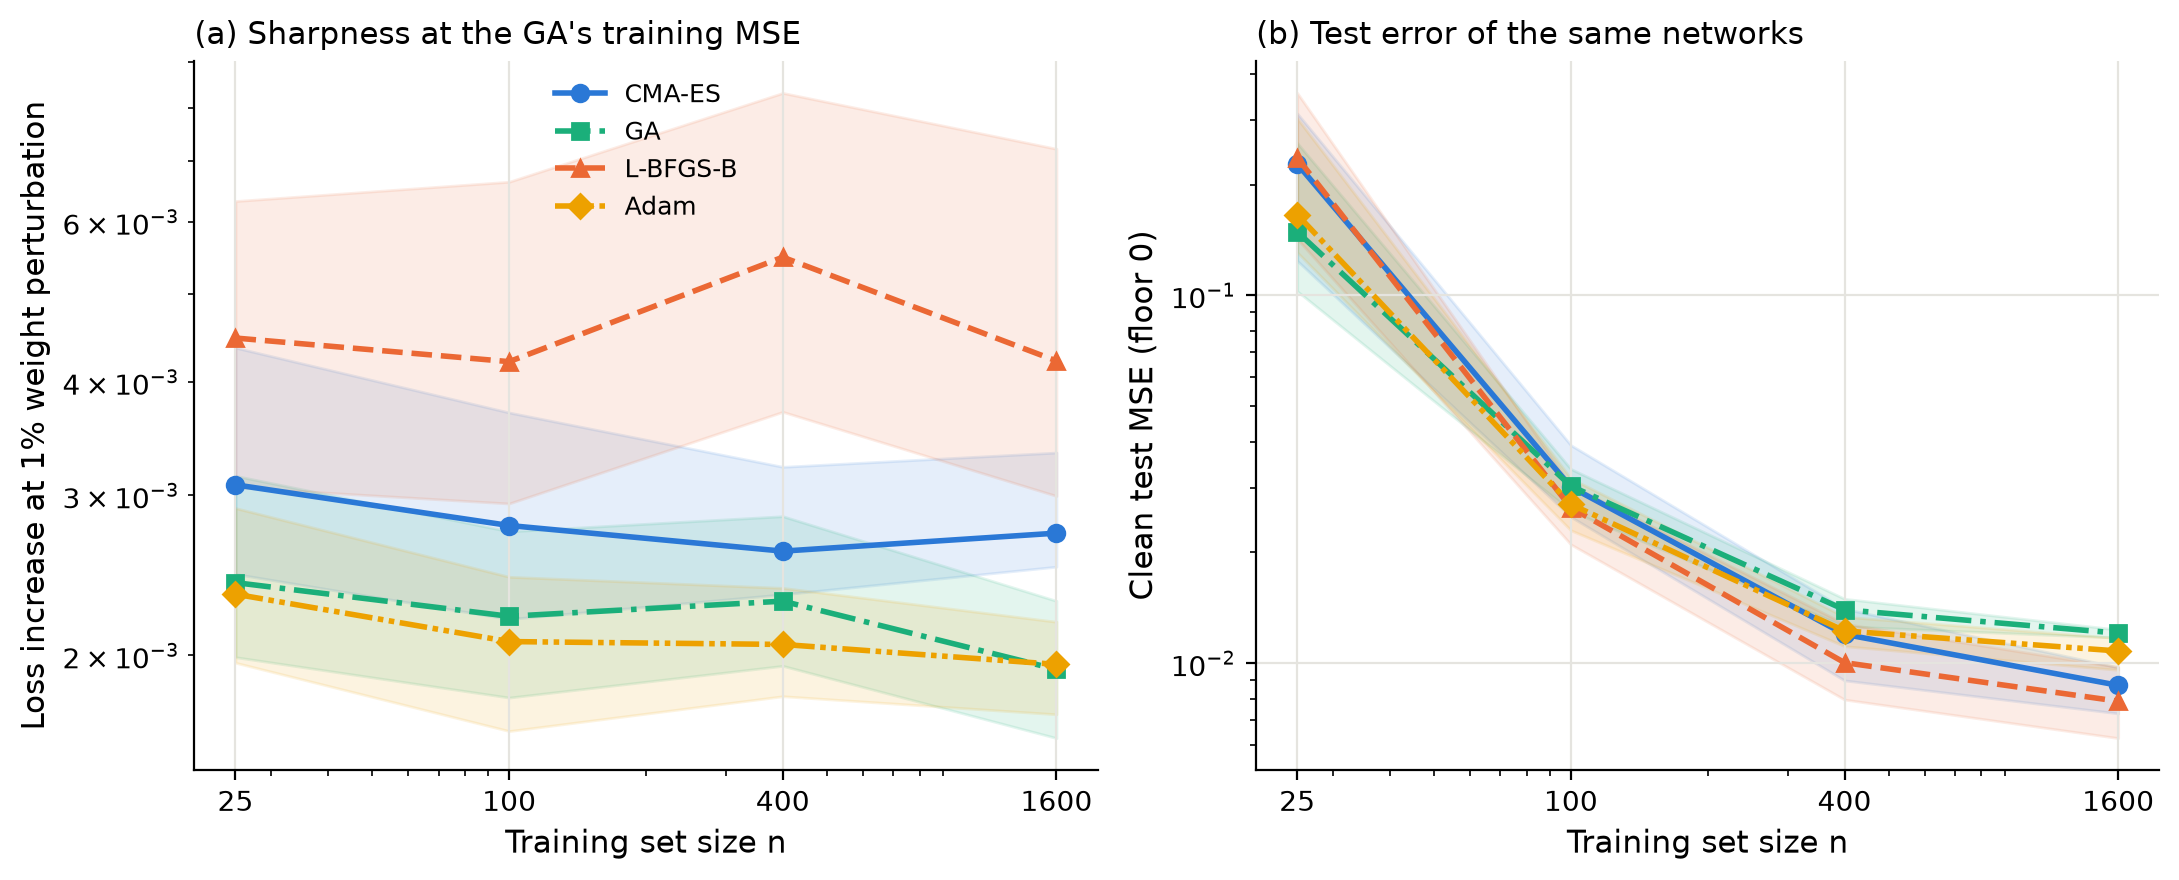
\includegraphics[width=\linewidth]{fig6_sharpness_matched.png}
  \caption{At matched training MSE (the GA's, per seed): (a) perturbation sharpness $S_{0.01}$ and (b) clean
  test MSE of the same networks.}
  \label{fig:sharp}
\end{figure}
\todo{Table with $\lambda_{\max}$ and weight norms next to $S_\rho$ (appendix), from
\texttt{p5\_selection/sharpness.csv}.}

\subsection{Choosing the hidden-layer size}
\label{sec:res-arch}
The assignment's extension asks whether an EA chooses a model size that tracks $n$. Evolving $H$ with the
validation error as fitness would turn the validation set into the EA's training data, which is unfair to
methods that fit on the training set, and a search over at most 20 values of $H$ is exhaustive anyway. We
therefore give every method the same capacity selection (\cref{sec:selection}) and report the chosen $H$ per
method (\cref{tab:arch,fig:arch}).

\begin{table}[t]
  \centering
  \caption{$H$ and early stopping chosen on the selection set: median clean test MSE / median chosen $H$
  (30 seeds, $H\in\{2,4,6,10,15,20\}$). Bold: not significantly worse than the best method at that $n$.}
  \label{tab:arch}
  \small
  \begin{tabular}{@{}r cccc@{}}
    \toprule
    $n$ & \cmaes & GA & \lbfgs & Adam \\
    \midrule
    25   & \textbf{0.100} / 10  & \textbf{0.102} / 15   & \textbf{0.119} / 10  & \textbf{0.106} / 10 \\
    100  & 0.024 / 10           & 0.026 / 12.5          & \textbf{0.019} / 6   & 0.024 / 6 \\
    400  & \textbf{0.0049} / 10 & 0.0115 / 15           & \textbf{0.0046} / 8  & 0.0057 / 6 \\
    1600 & \textbf{0.0012} / 10 & 0.0087 / 20           & \textbf{0.0013} / 10 & 0.0017 / 10 \\
    \bottomrule
  \end{tabular}
\end{table}

\begin{figure}[t]
  \centering
  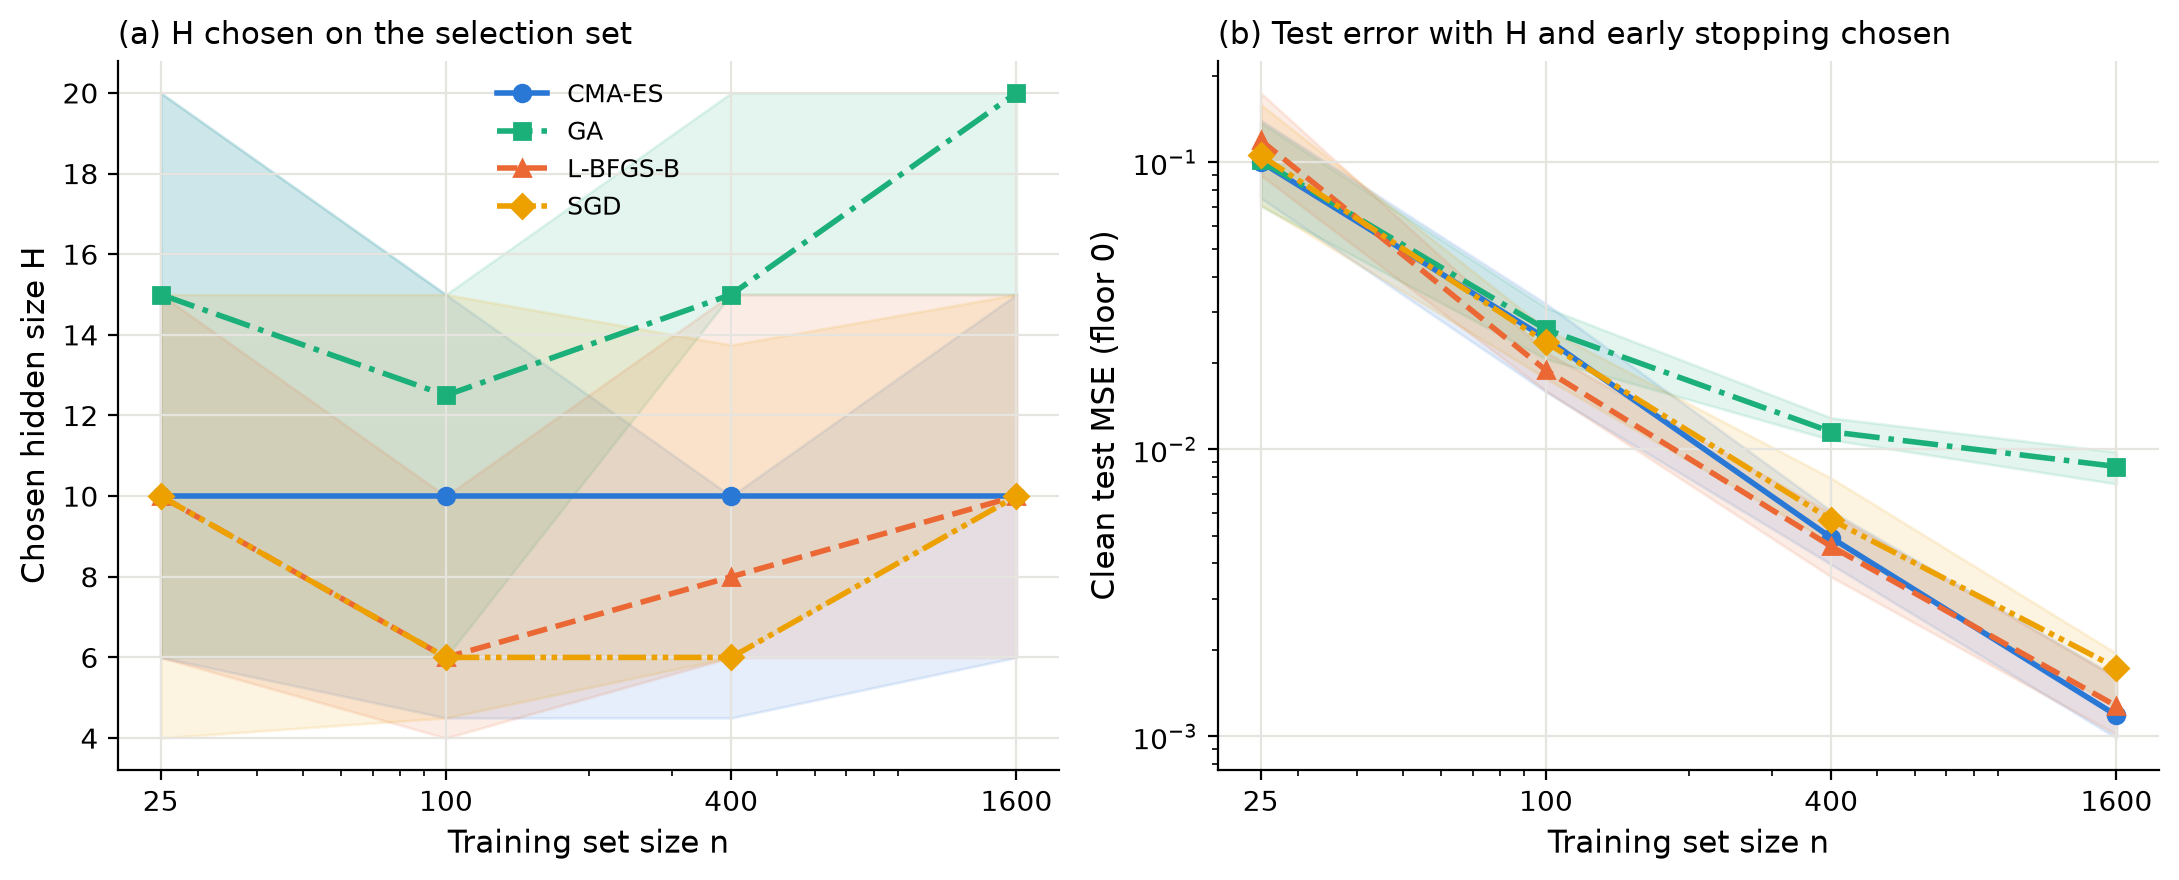
\includegraphics[width=\linewidth]{fig7_chosen_h.png}
  \caption{(a) Hidden size chosen on the selection set and (b) clean test MSE of the chosen networks vs.\ $n$.}
  \label{fig:arch}
\end{figure}

\begin{itemize}
  \item $n=25$: no significant differences. $n=100$: \lbfgs{} is best (beats \cmaes, GA and Adam,
  $p_{\mathrm{Holm}}\le0.031$). $n\ge400$: the GA is the worst ($\delta\ge0.87$); \cmaes{} and \lbfgs{} are best.
  \item Choosing $H$ improves on fixed $H=10$ in 9 of 16 (method, $n$) cells and is never significantly worse;
  the gain is largest for the GA at large $n$ ($0.012\to0.0087$ at $n=1600$). The ranking does not change.
  \item The chosen $H$ does not track $n$ cleanly: a selection set of $n$ points is noisy (wide IQRs). The GA
  chooses the largest networks (median 15--20 for $n\ge400$): extra capacity compensates its under-fitting.
\end{itemize}

% =============================================================================
\section{Discussion}
\label{sec:discussion}

\subsection{RQ1: better generalisation or only equal fit?}
\todo{Answer: at equal evaluations and with the lowest-training-loss network, the GA generalises much better at
small $n$, but it never fits as well as the others; \cmaes{} fits and generalises like the gradient methods.
Once all methods get the same early stopping and capacity selection, no EA generalises better: \cmaes{} is on
par, the GA is on par only at $n=25$ and worse from $n=100$ on. Under-fitting is the mechanism.}

\subsection{RQ2: dependence on the training-set size}
\todo{The pattern depends strongly on $n$: the GA's relative position goes from best ($n\le100$) to worst
($n=1600$) in the core sweep. Explain with the bias--variance trade-off: when $p/n$ is large, fitting less
is a regulariser; when $n$ is large, under-fitting costs more than over-fitting. With fair selection the
dependence on $n$ is mostly the GA's growing optimisation deficit.}

\subsection{H1: flat minima or implicit early stopping?}
\todo{H1 is not supported as a property of EAs: (i) the advantage comes with a higher training error
(falsification criterion 3); (ii) it vanishes under equal early stopping; (iii) at matched training error the GA
is flatter than \lbfgs{} but not than Adam, and flatness does not predict test error except at $n=25$ (consistent
with \citep{dinh2017sharp}). The pilot already showed that the EA's test error \emph{rises} with the budget.
Discuss the one place where H1 has support ($n=25$).}

\subsection{Cost}
\todo{Evaluations to the best (early-stopped) network: \lbfgs{} $10^2$--$10^3$, Adam $10^3$--$10^4$, \cmaes{}
$10^4$, GA $\ge10^5$; wall-clock per evaluation; why \cmaes{} is the far better EA here (correlated mutations
in 41 dimensions) and why the GA needs more than $10^6$ evaluations to fit as well.}

\subsection{When are EAs worth it for weight training?}
\todo{Non-differentiable or noisy objectives, discrete components, very small networks, parallel hardware;
for smooth regression with exact gradients a derivative-based method plus validation-based early stopping
is cheaper and at least as good. Relate to \citep{yao1999evolving,such2017deep}.}

\subsection{Threats to validity}
\begin{itemize}
  \item \textbf{Single problem and model:} one 2-D generator, one noise level, one architecture family.
  \item \textbf{Tuning at $H=10$, $n\in\{100,400\}$:} settings may be sub-optimal at other $H$ or $n$; the GA's
  winner sat at the edge of its grid twice.
  \item \textbf{Budget unit:} evaluations with $g=2$; checked with $g\in\{1,3\}$ and wall-clock time.
  \item \textbf{Bounds as regulariser:} 5--17\% of the non-GA weights sit at $\pm5$; the box acts differently on
  different methods.
  \item \textbf{Checkpoint grid:} early stopping can only stop at checkpoints (10 per decade).
  \item \textbf{Environment:} \cmaes{} results depend on the \texttt{cma}/numpy versions (a second machine gave
  different \cmaes{} runs with the same conclusions); all other methods reproduced bit-for-bit.
\end{itemize}
\todo{Expand each point by one sentence on its likely effect.}

% =============================================================================
\section{Limitations and future work}
\label{sec:limitations}
\todo{Noise sweep ($\sigma\in\{0.1,0.5\}$) and $d=5$ (extension E3); evolving weight decay (E2); larger networks
and real data sets; other EAs (IPOP-CMA-ES, NEAT); selection sets of other sizes; classification.}

% =============================================================================
\section{Conclusions}
\label{sec:conclusion}
\todo{3--5 sentences: the answer to RQ1/RQ2, the role of implicit early stopping, the practical recommendation.}

% =============================================================================
\bibliographystyle{plainnat}
\bibliography{references}

% =============================================================================
\appendix
\section{Decisions log}
\label{app:decisions}
\begin{table}[h]
  \centering
  \small
  \begin{tabularx}{\linewidth}{@{}l l X@{}}
    \toprule
    ID & Decision & Justification \\
    \midrule
    D1 & Regression, $f=\sin(\pi x_1)+\sin(\pi x_2)$ on $[-1,1]^2$ & exact noise floor; same smooth loss for all methods \\
    D2 & $\sigma=0.3$ (floor 0.09) & noisy enough for over-fitting to matter \\
    D3 & Budget in evaluations, gradient $=2$; wall-clock secondary & measured cost ratio 1.8--2.3; checked with 1, 3 and time \\
    D4 & $\B=10^5$; smaller budgets from snapshots & \cmaes{} training MSE changes $<1\%$ from 50k to 100k ($n\ge100$) \\
    D5 & $H=10$ (41 weights) & $p/n$ from 1.64 to 0.026; represents $f$ at $n=1600$ \\
    D6 & Return the lowest-training-loss network & isolates the optimiser; validation results logged \\
    D7 & 30 paired seeds; val/test data seed 10000 & paired non-parametric tests \\
    D8 & Independent random streams & initial weights never reuse the data's random numbers \\
    D9 & Equal tuning on training MSE, one edge extension & tuning on validation would reward under-fitting \\
    D10 & Selection set of $n$ points per run & realistic validation data; chooses only among trained networks \\
    D11 & Relative perturbation sharpness at matched training MSE & scale-aware; removes training progress \\
    \bottomrule
  \end{tabularx}
\end{table}

\section{Reproduction}
\label{app:repro}
\todo{Commands from \texttt{README.txt} (setup, core sweep, aggregation, figures, secondary experiments,
Phase 5) and the commits of each experiment: tuning \texttt{8ff680e}; Phase 4 \texttt{cbc64ec}; Phase 5.1
\texttt{ed67e33}; Phase 5.3 \texttt{e0294b4}.}

\section{Additional tables}
\todo{Full Wilcoxon tables (\texttt{results/processed/*/wilcoxon*.csv}), the full tuning table
(\texttt{tuning\_summary.csv}), $\lambda_{\max}$ and weight norms, chosen-$H$ counts (\texttt{chosen\_h.csv}).}

\end{document}
